\documentclass[11pt,letter]{article}
\usepackage{amsmath}
\usepackage{amssymb}	% packages that allow mathematical formatting
\usepackage{graphicx}	% package that allows you to include graphics
\usepackage{setspace}	% package that allows you to change spacing
\usepackage{fullpage}	% package that specifies normal margins
\usepackage{microtype}
\usepackage{amsthm}
\newcommand{\argmin}{\operatornamewithlimits{argmin}}
\renewcommand\qedsymbol{$\blacksquare$}
\usepackage{listings}
\usepackage{color}
\usepackage{subfig}


\definecolor{codegreen}{rgb}{0,0.6,0}
\definecolor{codegray}{rgb}{0.5,0.5,0.5}
\definecolor{codepurple}{rgb}{0.58,0,0.82}
\definecolor{backcolour}{rgb}{0.95,0.95,0.95}

\lstdefinestyle{mystyle}{
	backgroundcolor=\color{backcolour},   
	commentstyle=\color{codegreen},
	keywordstyle=\color{magenta},
	numberstyle=\tiny\color{codegray},
	stringstyle=\color{codepurple},
	basicstyle=\footnotesize,
	breakatwhitespace=false,         
	breaklines=true,                 
	captionpos=b,                    
	keepspaces=true,                 
	numbers=left,                    
	numbersep=5pt,                  
	showspaces=false,                
	showstringspaces=false,
	showtabs=false,                  
	tabsize=2
}

\lstset{style=mystyle}

%\usepackage[left=2.5cm, right=2.5cm, top=2cm, bottom = 3cm]{geometry}


	

\begin{document}

\begin{figure}
	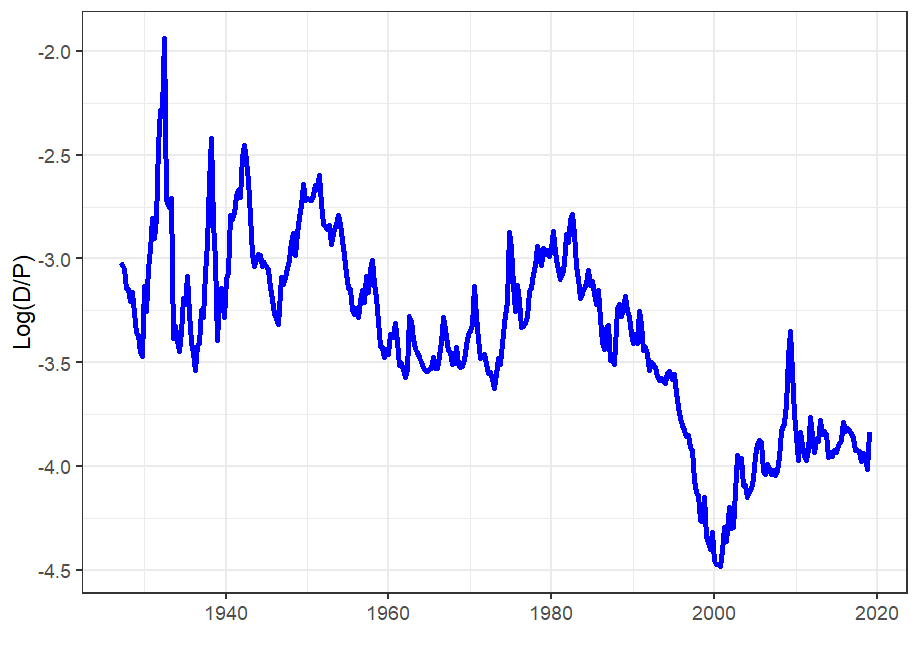
\includegraphics[width=\linewidth]{log_dividend_yield.png}
	\caption{Dividend yield (sum of past years worth of dividends divided by current portfolio price)}
	\label{fig:div_yield}
\end{figure}
We run two regressions separately of the form
\begin{equation*}
	\begin{split}
	r_{t, t+\tau} & = \alpha_r + \beta_{r, \tau}(d_t - p_t)\\
	\Delta d_{t, t+\tau} & = \alpha_{\Delta_d}+\beta_{\Delta d, \tau}(d_t - p_t)\\
	\end{split}
\end{equation*}
the results of which are shown in the tables below


\begin{table}[!htbp] \centering 
	\label{} 
	\begin{tabular}{@{\extracolsep{5pt}} cccc} 
		\\[-1.8ex]\hline 
		\hline \\[-1.8ex] 
		& b & se & r2 \\ 
		\hline \\[-1.8ex] 
		4 & $0.117$ & $0.902$ & $0.0001$ \\ 
		12 & $4.213$ & $1.086$ & $0.043$ \\ 
		20 & $8.075$ & $1.087$ & $0.107$ \\ 
		\hline \\[-1.8ex] 

	\end{tabular} 
	\quad
	\begin{tabular}{@{\extracolsep{5pt}} cccc} 
		\\[-1.8ex]\hline 
		\hline \\[-1.8ex] 
		& b & se & r2 \\ 
		\hline \\[-1.8ex] 
		4 & -$0.488$ & $0.106$ & $0.063$ \\ 
		12 &-$1.254$ & $0.202$ & $0.121$ \\ 
		20 &-$1.943$ & $0.291$ & $0.150$ \\ 
		\hline \\[-1.8ex] 
	\end{tabular} 
			\caption{Return Regressions (left panel) and dividend growth regressions (right panel)} 
\end{table} 




\end{document}


